\chapter{Dise�o de Interfaces}\label{appendix:mockupsApendix}
En este ap�ndice se muestran los dise�os realizados para cada una de las interfaces y los procesos visuales de la aplicaci�n.
\begin{figure}[htpb]
	\centering
	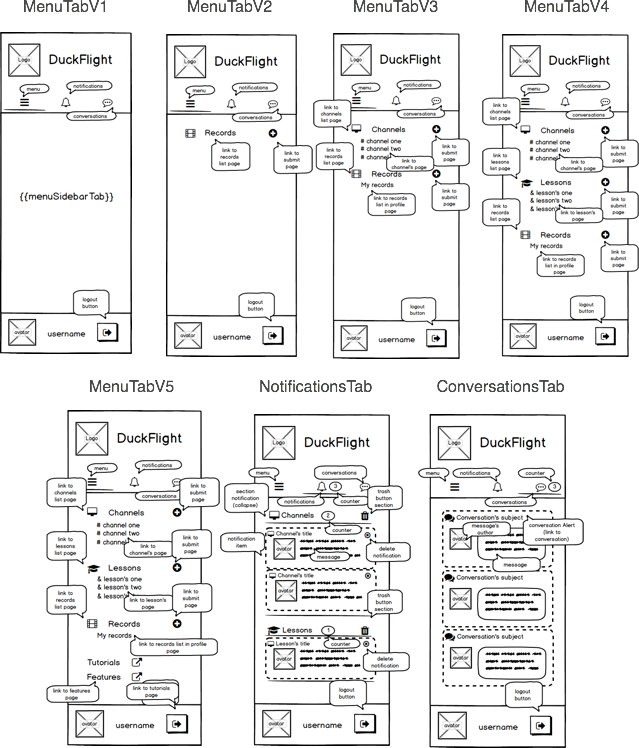
\includegraphics[width=0.7\textwidth]{sidebarVersions.png}
	\caption{Dise�o sidebar}
	\label{fig:sidebarVersions}
\end{figure}


\begin{figure}[h]
	\centering
	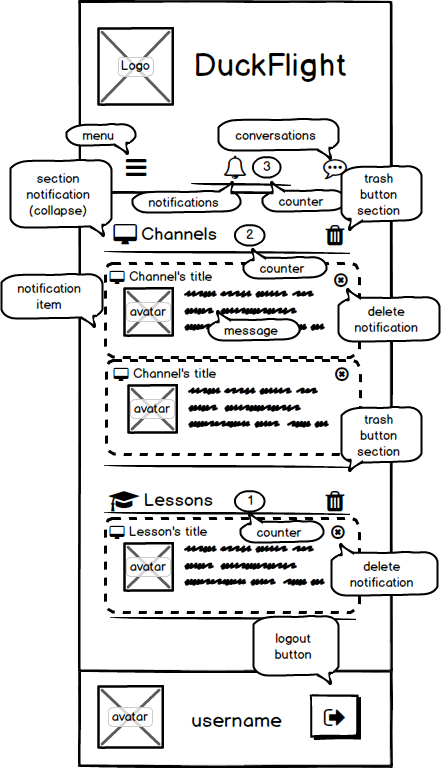
\includegraphics[scale=0.7]{sidebarNotifications.png}
	\caption{Dise�o pesta�a notificaciones para el sidebar}
	\label{fig:sidebarNotifications}
\end{figure}

\begin{figure}[h]
	\centering
	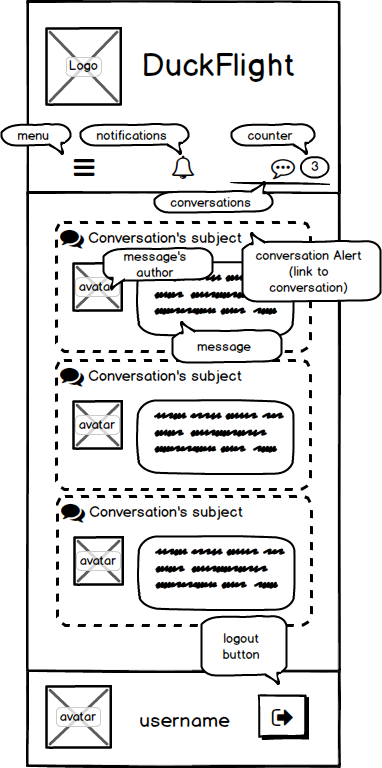
\includegraphics[scale=0.7]{sidebarConversations.png}
	\caption{Dise�o pesta�a conversaciones para el sidebar}
	\label{fig:sidebarConversations}
\end{figure}


\begin{figure}[h]
	\centering
	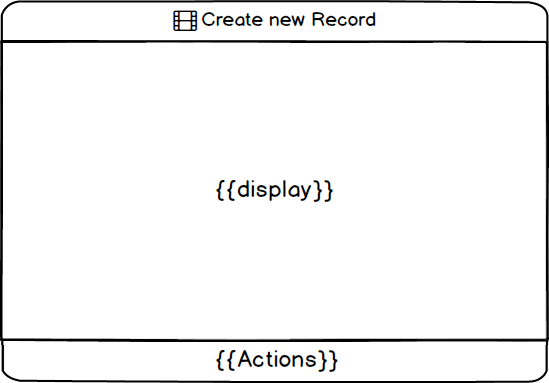
\includegraphics[width=0.9\textwidth]{recorderBase}
	\caption{Dise�o base grabador}
	\label{fig:recorderBase}
\end{figure}



\begin{figure}[h]
	\centering
	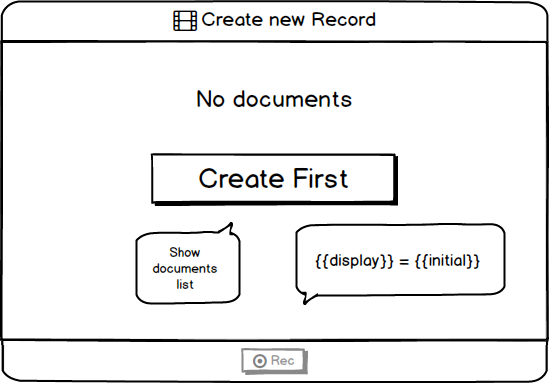
\includegraphics[width=0.9\textwidth]{recorderNoDocuments.png}
	\caption{Dise�o panel inicial grabador}
	\label{fig:recorderNoDocs}
\end{figure}

\begin{figure}[h]
	\centering
	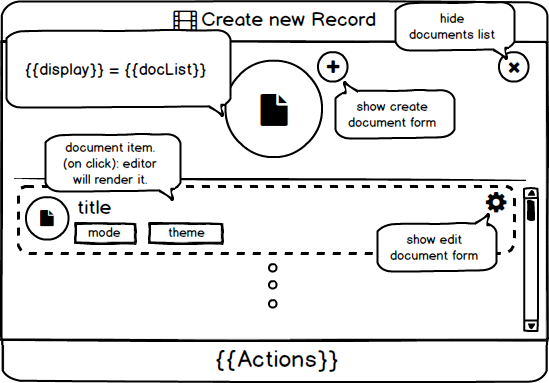
\includegraphics[width=0.9\textwidth]{recorderDocumentsList.png}
	\caption{Dise�o panel documentos en grabador}
	\label{fig:recorderDocsList}
\end{figure}

\begin{figure}[h]
	\centering
	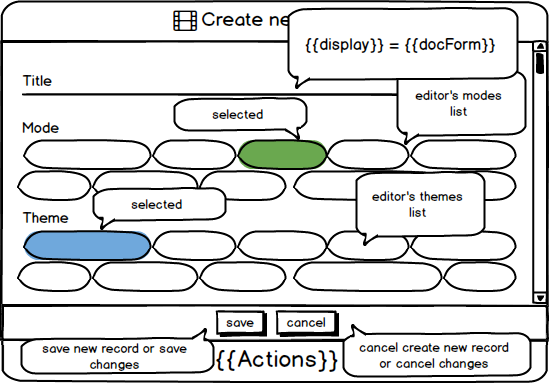
\includegraphics[width=0.9\textwidth]{recorderDocumentForm.png}
	\caption{Dise�o formulario documentos}
	\label{fig:documentForm}
\end{figure}

\begin{figure}[h]
	\centering
	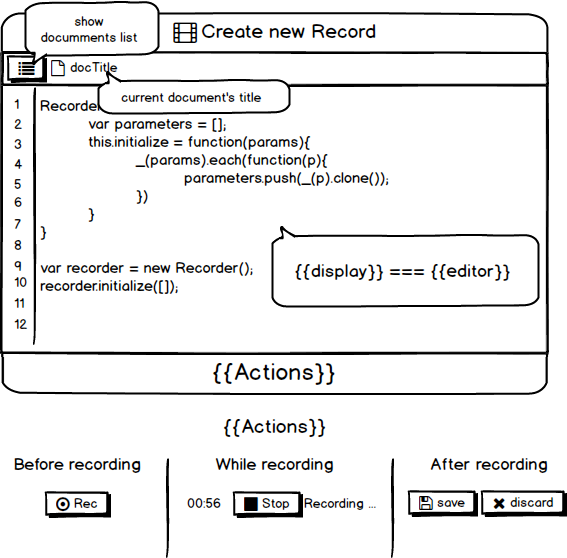
\includegraphics[width=0.9\textwidth]{recorderEditor.png}
	\caption{Dise�o editor en grabador}
	\label{fig:recorderEditor}
\end{figure}

\begin{figure}[h]
	\centering
	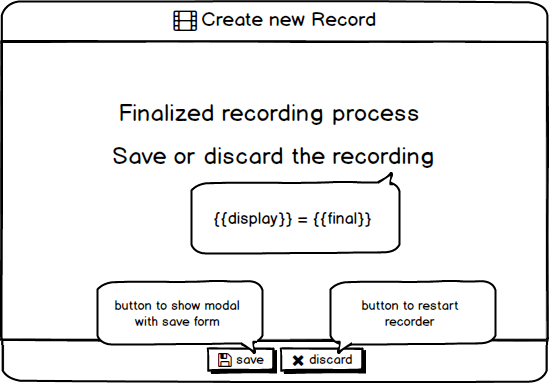
\includegraphics[width=0.9\textwidth]{recorderFinal.png}
	\caption{Dise�o final grabaci�n}
	\label{fig:recorderFinal}
\end{figure}

\begin{figure}[h]
	\centering
	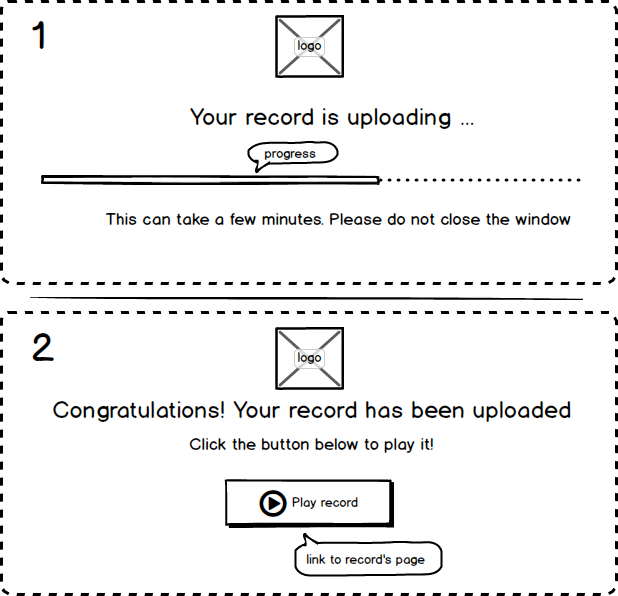
\includegraphics[width=0.9\textwidth]{recordUploadProcess.png}
	\caption{Dise�o proceso de subida}
	\label{fig:uploadProcess}
\end{figure}

\begin{figure}[h]
	\centering
	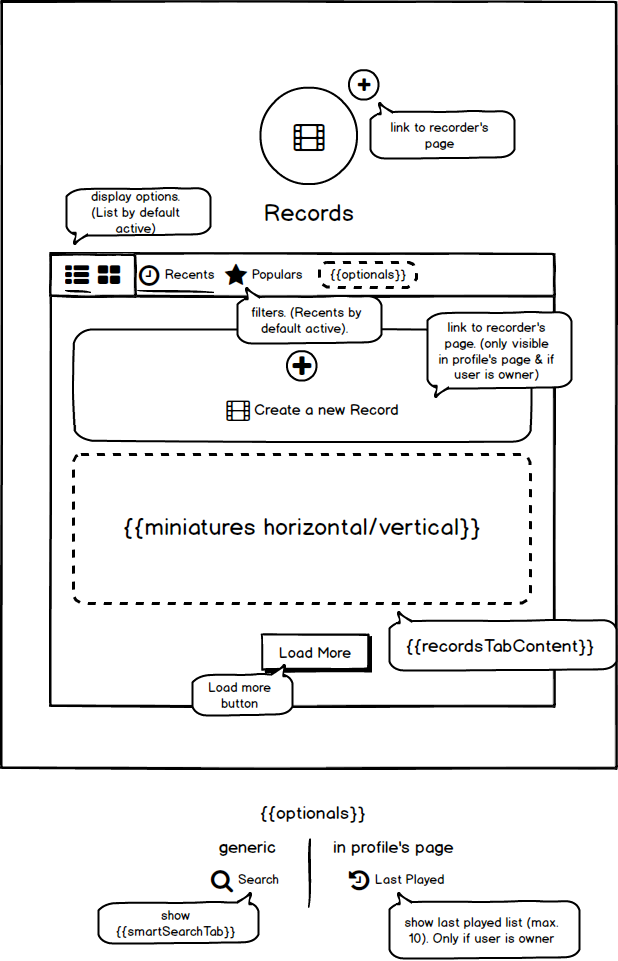
\includegraphics[width=0.8\textwidth]{recordsPage.png}
	\caption{Lista de grabaciones}
	\label{fig:recordsPage}
\end{figure}

\begin{figure}[h]
	\centering
	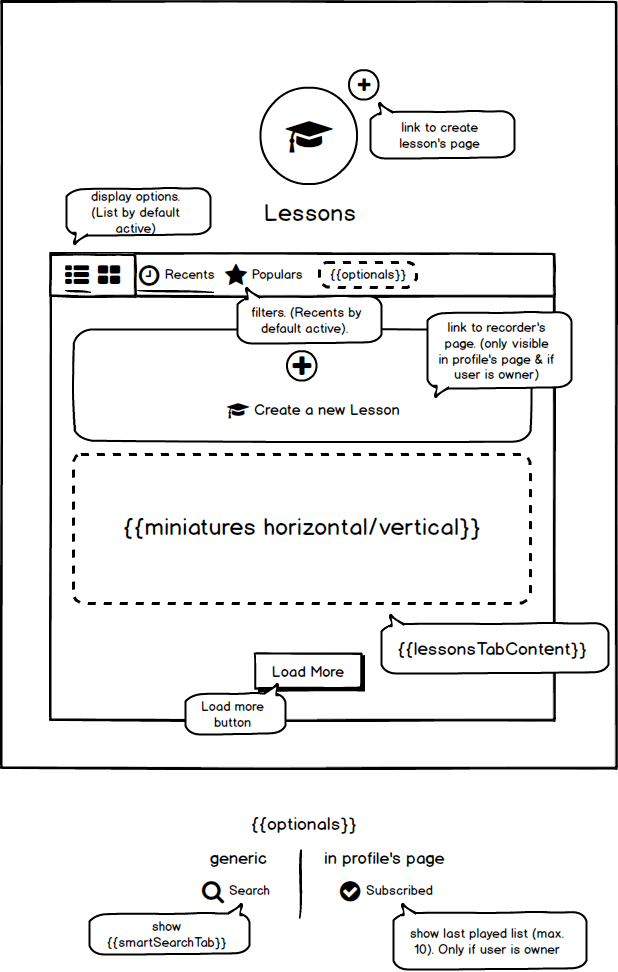
\includegraphics[width=0.8\textwidth]{lessonsPage.png}
	\caption{Lista de lecciones}
	\label{fig:lessonsPage}
\end{figure}

\begin{figure}[h]
	\centering
	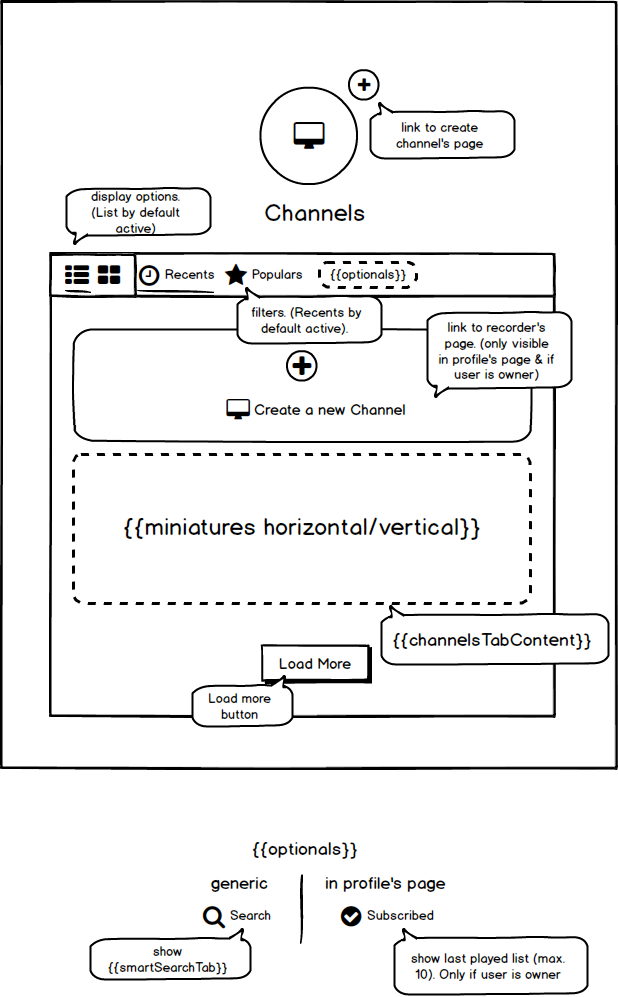
\includegraphics[width=0.8\textwidth]{channelsPage.png}
	\caption{Lista de canales}
	\label{fig:channelsPage}
\end{figure}

\begin{figure}[h]
	\centering
	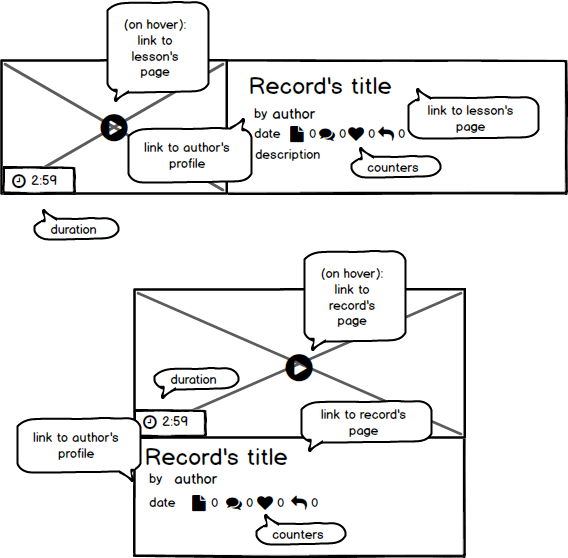
\includegraphics[width=0.8\textwidth]{miniaturesRecord.png}
	\caption{Miniatura grabaci�n}
	\label{fig:miniaturesRecord}
\end{figure}

\begin{figure}[h]
	\centering
	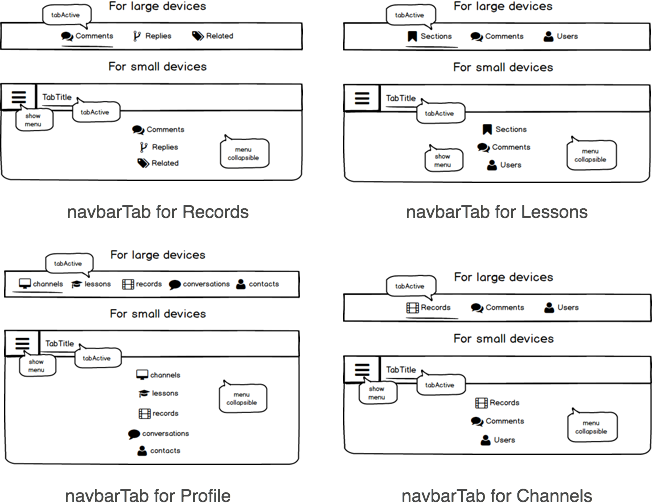
\includegraphics[width=0.8\textwidth]{navbarTabDesign.png}
	\caption{Dise�o de navbarTab}
	\label{fig:navbarTabDesign}
\end{figure}

\begin{figure}[htpb]
	\centering
	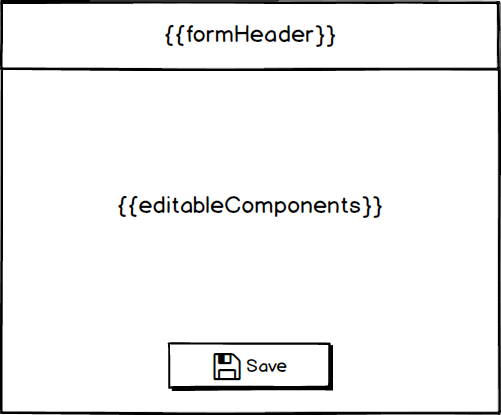
\includegraphics[width=0.8\textwidth]{editFormBase.png}
	\caption{Dise�o base para el formulario de edici�n}
	\label{fig:editFormBase}
\end{figure}

\begin{figure}[htpb]
	\centering
	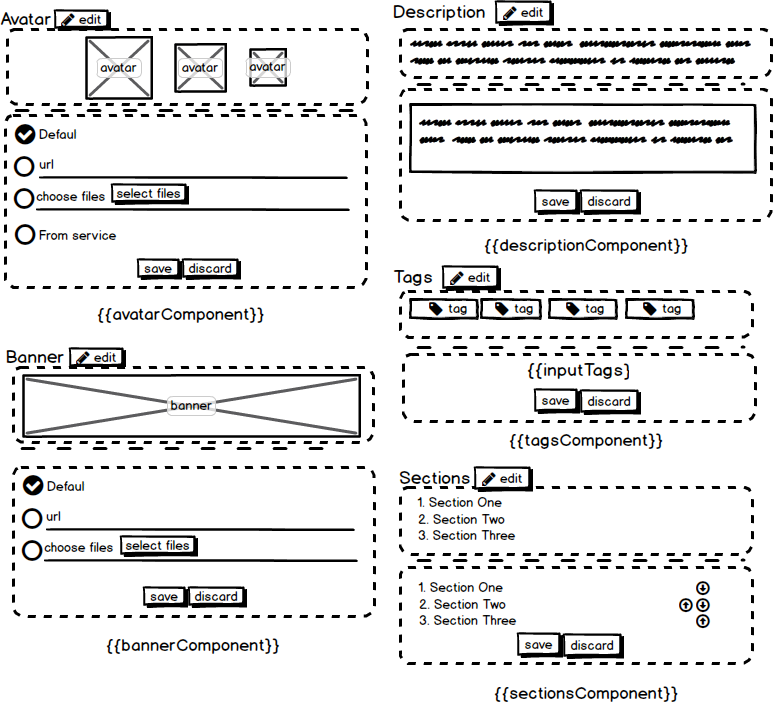
\includegraphics[width=0.8\textwidth]{formEditComplements.png}
	\caption{Dise�o componentes del formulario de edici�n}
	\label{fig:formEditComplements}
\end{figure}

\begin{figure}[htpb]
	\centering
	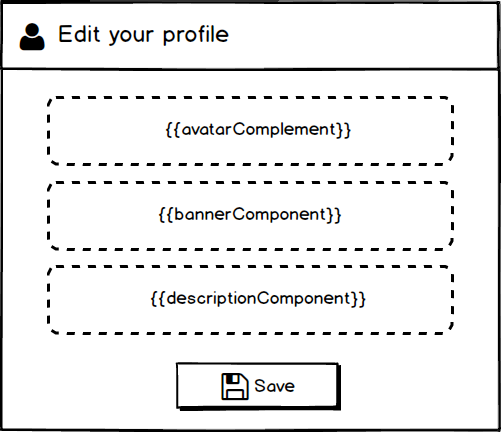
\includegraphics[width=0.8\textwidth]{profileEdit.png}
	\caption{Formulario de edici�n del perfil}
	\label{fig:profileEdit}
\end{figure}

\begin{figure}[h]
	\centering
	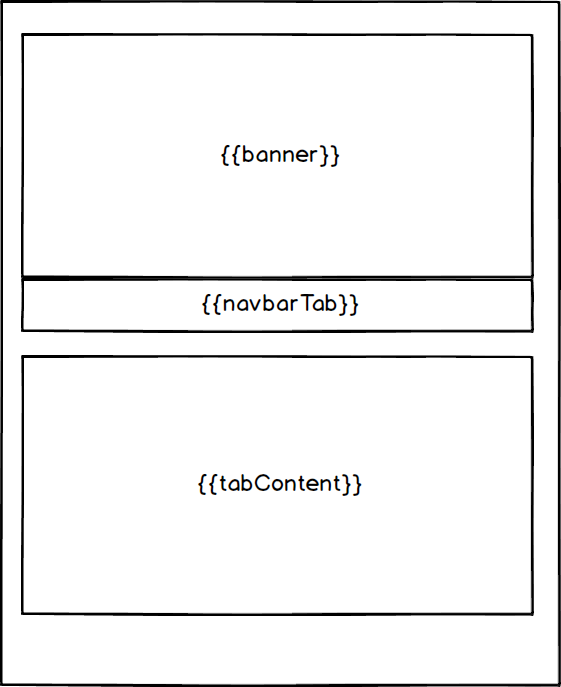
\includegraphics[width=0.5\textwidth]{pageDetailBase.png}
	\caption{Dise�o p�gina de detalle}
	\label{fig:detailBase}
\end{figure}

\begin{figure}[htpb]
	\centering
	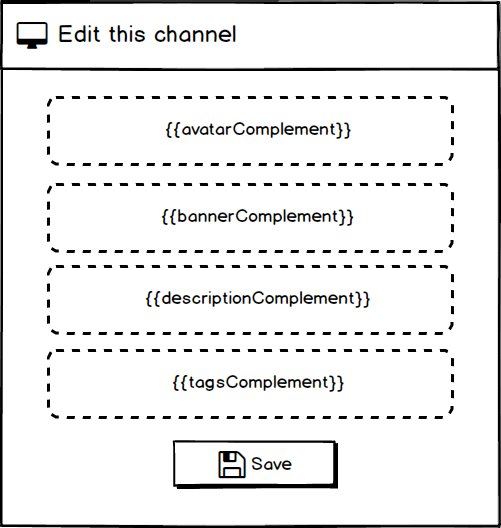
\includegraphics[width=0.8\textwidth]{channelEdit.png}
	\caption{Formulario de edici�n de un canal}
	\label{fig:channelEdit}
\end{figure}

\begin{figure}[htpb]
	\centering
	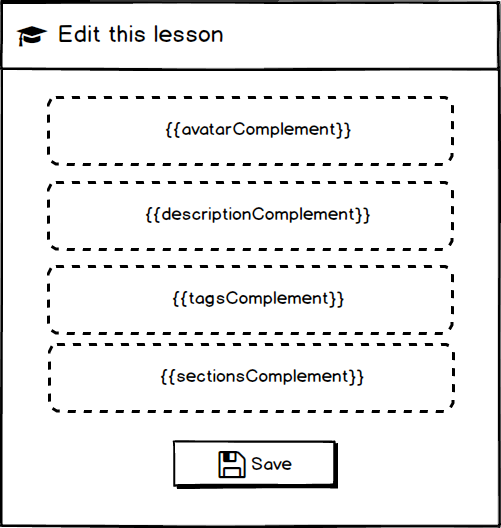
\includegraphics[width=0.9\textwidth]{lessonEdit.png}
	\caption{Formulario de edici�n de una lecci�n}
	\label{fig:lessonEdit}
\end{figure}

\begin{figure}[htpb]
	\centering
	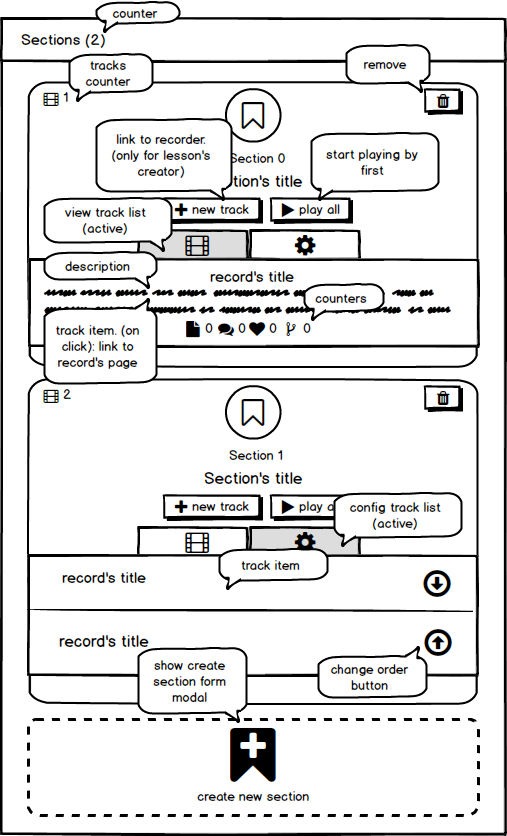
\includegraphics[width=0.9\textwidth]{sectionsTab.png}
	\caption{Dise�o de la pesta�a de secciones}
	\label{fig:sectionsTab}
\end{figure}

\begin{figure}[htpb]
	\centering
	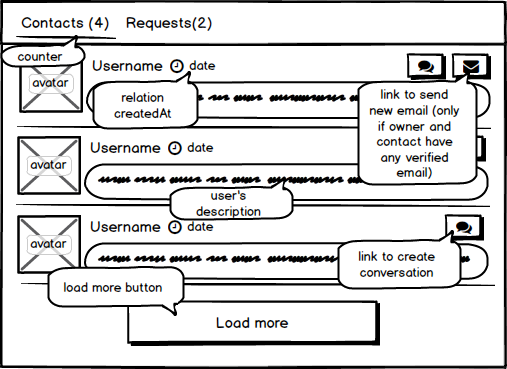
\includegraphics[width=0.9\textwidth]{contactsTab.png}
	\caption{Lista de contactos}
	\label{fig:contactsTab}
\end{figure}

\begin{figure}[htpb]
	\centering
	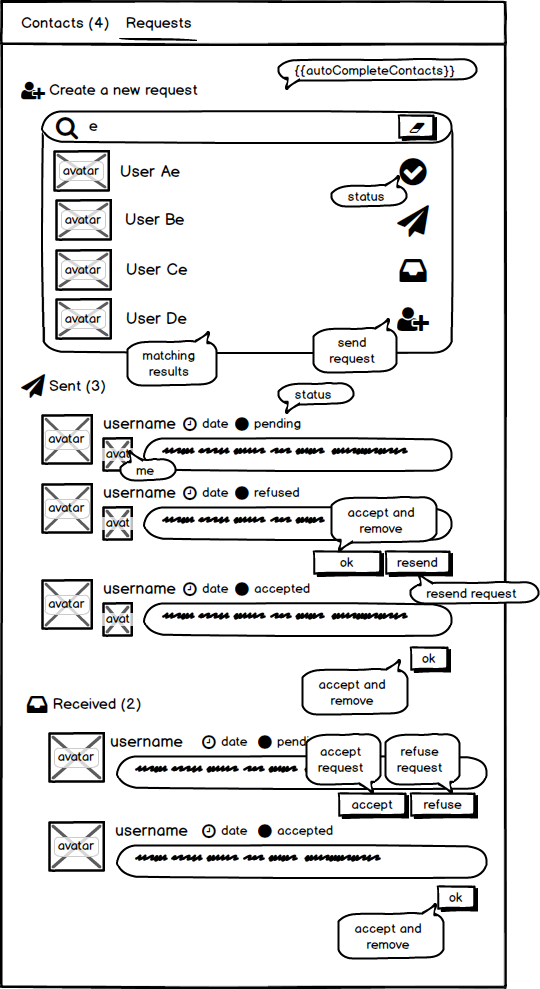
\includegraphics[width=0.7\textwidth]{requestsTab.png}
	\caption{Peticiones de contacto}
	\label{fig:requestsTab}
\end{figure}

\begin{figure}[htpb]
	\centering
	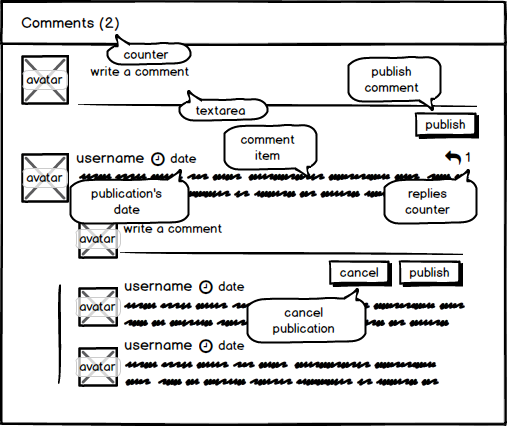
\includegraphics[width=0.9\textwidth]{commentsTab.png}
	\caption{Espacio para comentarios}
	\label{fig:commentsTab}
\end{figure}

\begin{figure}[htpb]
	\centering
	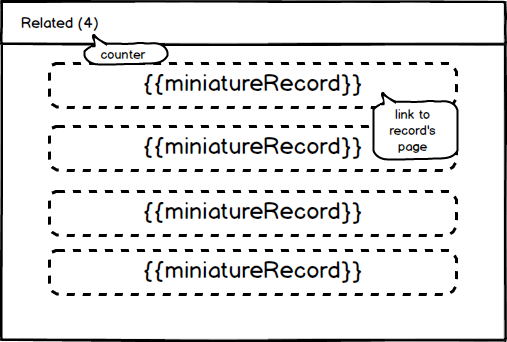
\includegraphics[width=0.9\textwidth]{relatedTab.png}
	\caption{Lista de relacionados}
	\label{fig:relatedTab}
\end{figure}

\begin{figure}[htpb]
	\centering
	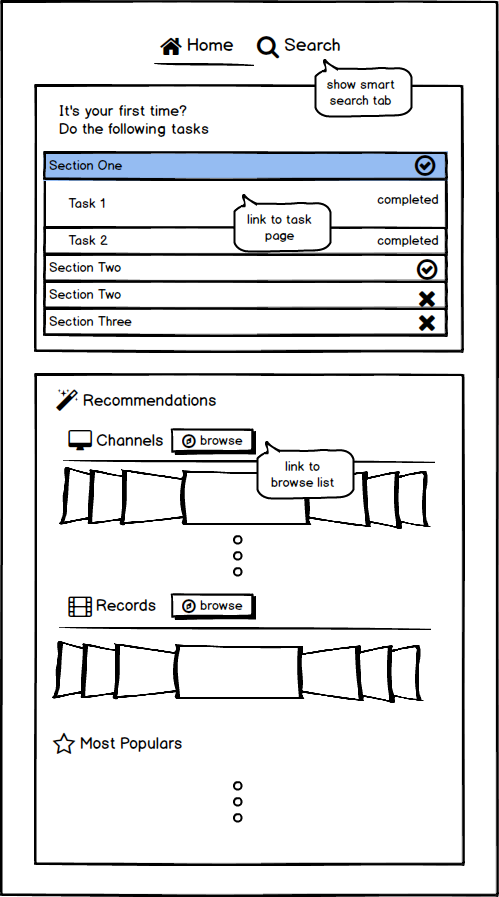
\includegraphics[width=0.8\textwidth]{mainPage.png}
	\caption{Dise�o de la p�gina principal}
	\label{fig:mainPage}
\end{figure}


\begin{figure}[htpb]
	\centering
	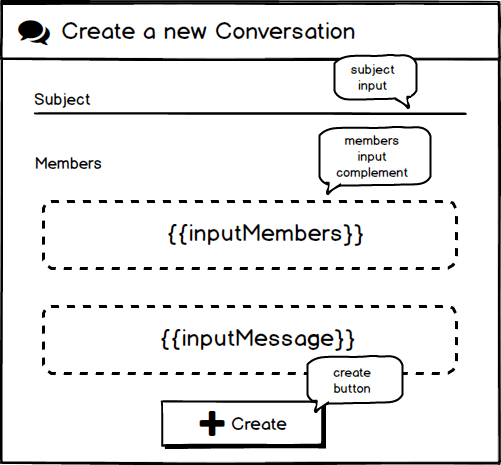
\includegraphics[width=0.8\textwidth]{createConversation.png}
	\caption{Dise�o del formulario de creaci�n para las conversaciones}
	\label{fig:createConversation}
\end{figure}
\begin{figure}[htpb]
	\centering
	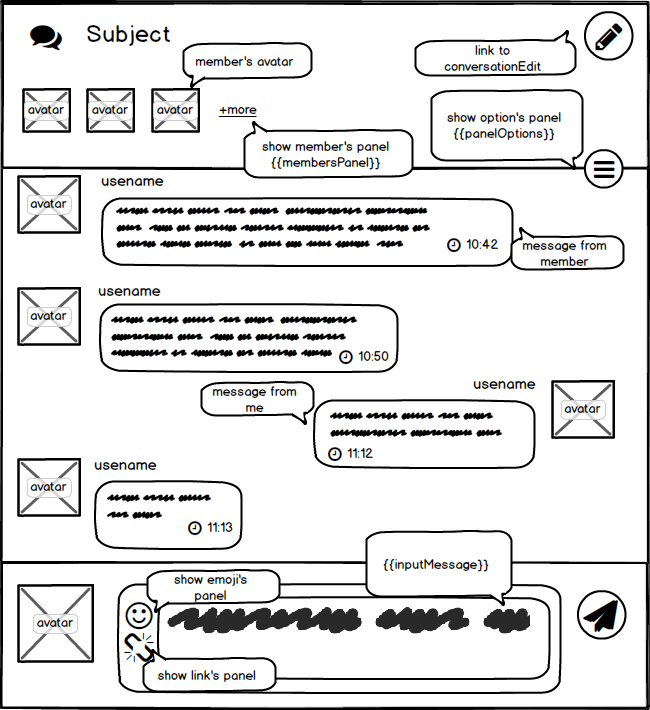
\includegraphics[width=0.8\textwidth]{conversationDesign.png}
	\caption{Dise�o de la p�gina de una conversaci�n}
	\label{fig:conversationDesign}
\end{figure}
\begin{figure}[htpb]
	\centering
	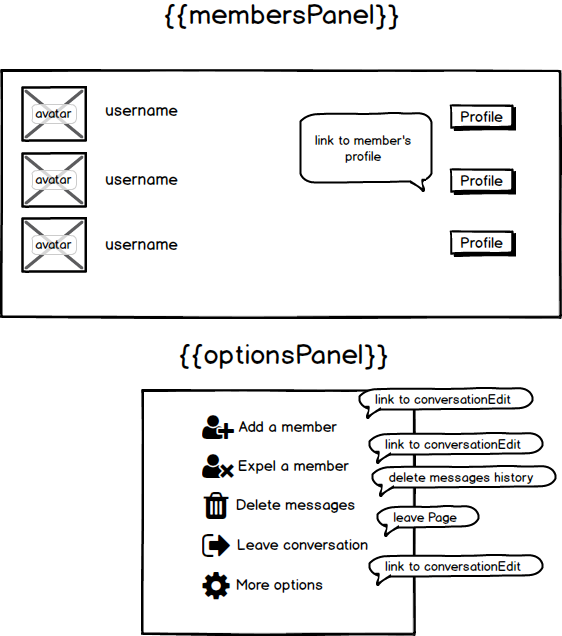
\includegraphics[width=0.8\textwidth]{conversationPanels.png}
	\caption{Paneles de la p�gina de conversaci�n}
	\label{fig:conversationPanels}
\end{figure}
\begin{figure}[htpb]
	\centering
	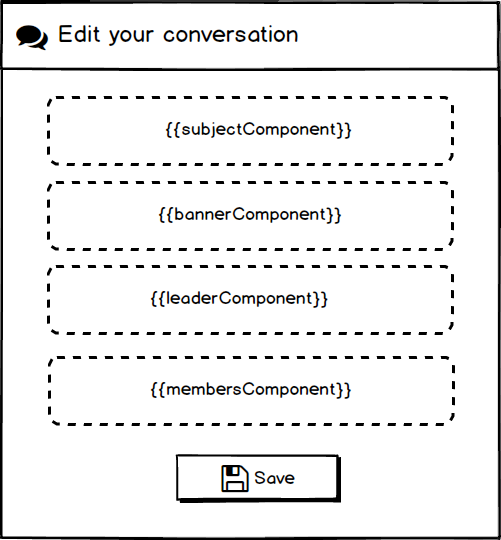
\includegraphics[width=0.8\textwidth]{conversationEdit.png}
	\caption{Dise�o formulario de edici�n de una conversaci�n}
	\label{fig:conversationEdit}
\end{figure}
\begin{figure}[htpb]
	\centering
	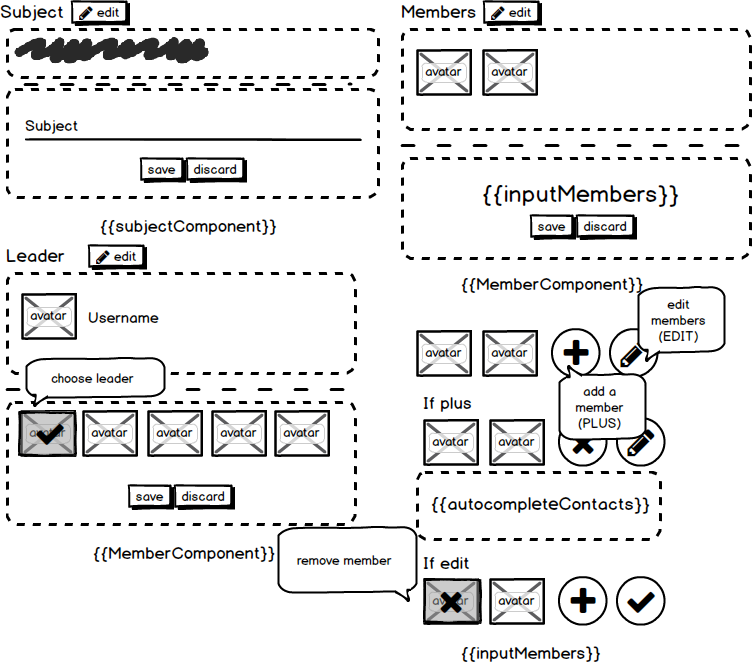
\includegraphics[width=0.8\textwidth]{conversationComplements.png}
	\caption{Dise�o de componentes para los formularios de una conversaci�n}
	\label{fig:conversationComplements}
\end{figure}







